\subsection{Raspberry Piをリモコンにしよう}

Raspberry Piにも赤外線を送ったり、受け取ることができるセンサーがついています。これを使って何ができるでしょうか?Raspberry Piをリモコンにして家電を制御することができます。

\begin{itemize}
\item リモコンをひとつにまとめることができる
\item 外出先から家電を操作することができる
\item 音声を使って家電を操作することができる
\end{itemize}

Raspberry Piをリモコンにするためには、リモコンの真似をすることが必要です。リモコンから赤外線の信号をセンサーボードの赤外線受信ユニットで受け取ります。コマンドを使って信号をテキストに変換します。変換された信号を赤外線センサーから家電に送信することで、リモコンと同じ信号を家電に送ることができます。

\begin{figure}[H]
    \centering
 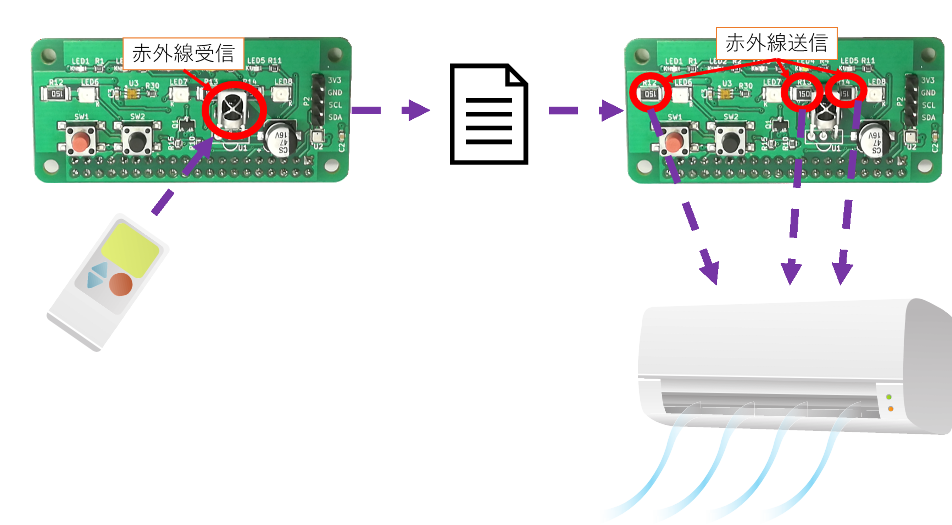
\includegraphics[scale=0.4]{images/chap05/text05-img041.png}
    \caption{Raspberry Piをリモコンにする手順}
\end{figure}

\begin{tcolorbox}[title=\useOmetoi]
ターミナルを開いて、コマンドを入力しましょう。
\begin{enumerate}
\item リモコンの信号を受け取り、ファイルに記録します。
 \begin{enumerate}[1]
  \item /home/pi/ome/05に移動します。\\ \code{cd /home/pi/ome/05}
  \item 違う信号を受け取らないように、赤外線受信を止めます。 \\ \code{sudo service lircd stop}
  \item 赤外線を受信し、onoff.txtに記録します。コマンドを実行してから、赤外線受信ユニットに向かって、リモコンのボタンを押しましょう。記録が終わったらCtrl+c(Ctrlキーを押しながらcを押す)で終了します。\\ \code{mode2 -d /dev/lirc0 | tee onoff.txt}
  \item 記録した信号を、convert\_pattern コマンドを使って送信用に変換します。\\ \code{convert\_pattern onoff.txt > onoff.pattern}
  \item 設定ファイルを作ります。/home/pi/ome/05/template.lircd.confを元に作ります。まずはこのテンプレートを05.lircd.confという名前でコピーします。そのあと、leafpadで開きましょう。\\ \code{cp template.lircd.conf 05.lircd.conf\\leafpad 05.lircd.conf}
  \item \pageref{template.lircd.conf}ページにあるリスト \ref{template.lircd.conf}の赤字の部分を書き換えます。
  \begin{enumerate}[(1)]
    \item リモコンの名前を決めます。使う家電の名前(fan, robot, TV...)にしましょう。
    \item 信号の名前を決めます。動作(digital\_onoff,walk...)の名前にしましょう。
    \item “ここに信号をペーストする”と書いてある行を消します。onoff.patternに書かれた信号をコピーして貼り付けます。leafpadを使ってonoff.patternを表示しましょう。\\ \code{leafpad onoff.pattern}
\\onoff.patternに書かれた信号は、たとえば「1207 588 447 838 447 823 475 812 1218」のような文字列です。\\書き換えたら、保存しましょう (名前が05.lircd.confになっていることを確認しましょう)。
  \end{enumerate}
 \end{enumerate}
\item ファイルに記録された信号を、赤外線LEDから送信する。
 \begin{enumerate}[1]
  \item 設定ファイルをコピーします。 \\ \code{sudo cp 05.lircd.conf /etc/lirc/lircd.conf.d/}
  \item 設定ファイルを再読み込みします。\\ \code{sudo service lircd restart}
  \item 赤外線を送ります。fanは設定ファイルに書いたリモコンの名前、onoffは設定ファイルに書いた信号の名前に変えましょう。\\ \code{irsend SEND\_ONCE \textcolor{red}{fan onoff}}
 \end{enumerate}
\end{enumerate}
\end{tcolorbox}

convert\_pattern コマンドは、mode2 コマンドの出力を送信用に変換しますが、このとき信号長 (信号列の数) を 256 個で打ち切っています。これは赤外線デバイスのドライバの制約によるものです\footnote{https://github.com/raspberrypi/linux/issues/3002 にてこの件に関する議論がなされています。新しいバージョンでは信号列長 1024 まで対応していますが、この講座で使うドライバには適用されていません。}。講座で使用する赤外線家電を使う上では支障ありませんが、おうちの家電に応用するときは注意する必要があります。たとえば、多くのエアコンの赤外線信号は信号長が長すぎてこの講座のプログラムをつかえません。\\
\begin{lstlisting}[caption=template.lircd.conf,label=template.lircd.conf]
begin remote

        name <#red#fan#>
        flags RAW_CODES
        eps 30
        aeps 100

        gap 200000
        toggle_bit_mask 0x0

        begin raw_codes
        name <#red#onoff#>
<#red#ここに信号をペーストする#>
        end raw_codes

end remote
\end{lstlisting}

\begin{figure}[H]
    \centering
 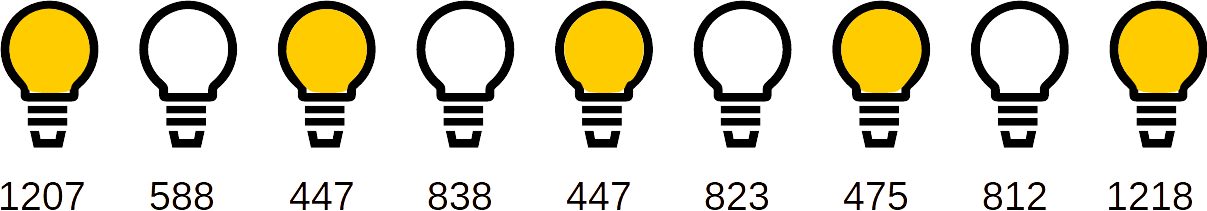
\includegraphics[width=\columnwidth]{images/chap05/text05-img042.png}
    \caption{信号のイメージ 数字にある時間で点灯/消灯が切り替わる}
\end{figure}